\chapter{Design}
\label{sec:design}
In this chapter the design for the Camera Provisioning system will be laid out.
The goal of the system is to provide a solution which makes it possible to manage camera configurations.
The system allows the user to orchestrate parameters into different templates which can be assigned to a camera.
The design will contain both functional and technical specifications containing the descriptions of different components, requirements and supplemental diagrams and wireframes.
\section{Requirements}
In table \ref{tab:requirements} the requirements for the system have been defined. Requirements are tracked using an identifier starting with a letter followed by a
number and are listed in the ID column of table \ref{tab:requirements}. If the identifier starts with the letter 'B' or a 'U' they specify a business or user requirement respectively. If the identifier starts with a 'F' or 'NF' they specify a functional or non-functional system requirement respectively.
Requirements have been prioritized using the MoSCoW method \cite{noauthor_moscow_nodate}.
\begin{table*}[h]
    \centering
    \begin{tabulary}{\linewidth}{CLL}
        \textbf{ID} & \textbf{Requirement} & \textbf{MoSCoW}
    %%% Business requirements
        \\ \hline %% Check this with NF-7
        B1 & A camera can be configured by the user without detailed technical knowledge about the model being used & Must
        \\ \hline
        B2 & A camera configuration can be rolled back to any compatible version in history & Must
        \\ \hline
        B3 & The configuration changes must include auditing: show the author and timestamp & Must
        \\ \hline
        B4 & Parameters whose values behave differently across brands shall be scaled by an adjustable factor for each brand & Should
        \\ \hline
        B5 & The application has the option to show the user the differences between the config in the camera and the template & Must
    %%% User requirements
        \\ \hline
        U1 & The interface must only allow authorized users, preferably via username and password & Could
        \\ \hline
        U2 & A user can change his credentials through the web interface & Could
        \\ \hline
        U3 & The template used for configuring cameras must include one setting representing a text-field and one setting representing a slider value & Should
        \\ \hline
        U4 & New settings can be added to the application without having to change the templates & Must
        \\ \hline
        U6 & The application should be able to handle one or more settings in a template that are not present in any of its parents & Should
        \\ \hline
        U7 & The user should be able to change templates via a user interface & Should
        \\ \hline
        U8 & A user can create a new template with a specified parent template & Must
        \\ \hline
        U9 & A user shall be able to trigger the configuration on one or all cameras according to their template & Must
		\\ \hline
		U10 & The user should be able to configure cameras via a user interface & Should
		\\ \hline
		U11 & The user must be able to assign which template a camera is associated with & Must
    %%% System requirements
        \\ \hline
        NF1 & The application must communicate with the cameras using HTTP & Must
        \\ \hline
        NF2 & The code must be compiled crossplatform & Must
        \\ \hline
        NF3 & The codebase must be covered with linting. & Must
        \\ \hline
        NF3 & The codebase shall be strongly typed. & Should
        \\ \hline
        NF3 & 90\% of code that does not interface with external systems shall be covered by unit tests& Must
        \\ \hline
        NF4 & Templates and camera configuration are stored on disk in a human-readable/writeable format & Must
        \\ \hline
        NF6 & The application is to be exposed as a REST API and documented via OpenAPI & Could
		\\ \hline
		NF7 & The application can be used interactively & Must
        \\ \hline
        NF8 & The templates must be camera independent. & Must
    \end{tabulary}
    \caption{Requirements}
    \label{tab:requirements}
\end{table*}

\section{General design}
At the conclusion of this project the prototype is handed over to the back-end team of BauWatch.
Since they will be further developing the prototype into a production ready system the choice was made to implement the system in Go as that programming language is their preferred language for new products fulfilling requirement NF-2.

\section{Templates}
The provisioning server will have a user interface through which a template can be configured.
A template in the context of this system is a collection of lists containing camera configuration options.
Templates can be built up from different layers where each layer can override parameters from the layer above.
This allows the user to define a template that is shared by a large amount of cameras but still allows fine-grained control over a smaller subset when this is desired.
These cameras would still use all the settings from the parent template but would have a different setting for the parameter being overridden.

\section{Datastructure}
Templates are represented in memory as a tree using dynamically allocated nodes that have pointers to one parent and zero or more children.
There is a single template that is considered to be the root node of the tree.
All templates that are added to the system will be a child of this root node.
The choice to represent the collection of templates as a tree is to solve the requirement of parameter inheritance.
Using this datastructure is an efficient method to enumerate the values of a template's parameters at configuration time.

A parameter can be enumerated by traversing each parent node starting from the node representing the current template and checking if it defines the sought parameter.
This process is repeated until a value for a given parameter is found.
Figure \ref{fig:find_param} shows how parameters are inherited.
If ParamB would be enumerated at Child2 the system would determine that it is not defined in Child2.
The system would then visit the parent nodes until a definition of ParamB is found.
Parameters A and C can be enumerated instantly since they are defined in Child2 itself where ParamC is newly introduced and ParamA overrides the values from Child1 and BaseTemplate.
\begin{marginfigure}
	\centering
	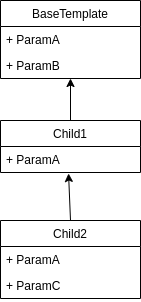
\includegraphics[width=3cm]{find_param}
	\caption{Parameter enumeration}
	\label{fig:find_param}
\end{marginfigure}
The best-case performance for a parameter lookup is O(1) in the case the parameter is already defined in the current template.
The worst-case performance of a lookup is O(n) where n is the number of templates to be traversed from the current node to the root node.
When a new template is instantiated, by creating a new one or loading one from YAML, that template has to be inserted at the correct place inside the tree.
The way this is achieved is to do a breadth-first search (BFS) in the tree where a match is identified using the name of the parent node.
Using BFS to find the parent node is more efficient than a depth-first search (DFS) as a template is more likely to inherit from a more generic template describing e.g. parameters for a country than a more specific template representing parameters for a specific building site. % TODO Proof?

\section{Multiple base templates} %TODO: Root template requires more intro?
While this design requires a single root template that all other templates inherit from, the design still allows the creation of multiple trees with independent parameter sets as can be seen in figure \ref{fig:multiple_root}.
This can be done by not setting any parameters in the root template such that the templates directly below it don't have any parameters that can be inherited from the root template.
The children of the root template then become the first template to define the template effectively turning into root templates themselves while still being children of the actual root template.
\begin{marginfigure}
	\centering
	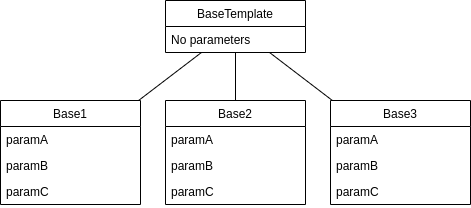
\includegraphics{multiple_root}
	\caption{Defining multiple base templates}
	\label{fig:multiple_root}
\end{marginfigure}

\section{Parameters}
Cameras can contain many different types of parameters.
These parameters can consist of something simple like an integer or a text string but they can also be represented as something more complex like a bitmap representing a section of a rectangle.
To allow a template to work with these parameters in a generic way some abstractions can be applied.
Templates contain a map of which the key is a string representing the name of a parameter and the value is a pointer to an object implementing the parameter interface.
As can be seen in figure \ref{fig:class_diagram} there are three parameters implementing the parameter interface.
These are the classes IntegerParameter, StringParameter and LevelParameter.
This way the template class can expose access to its parameters to the CameraAPI without needing to concern itself with what the type of its parameters are.
The Get and Set method of the Parameter interface behave differently depending on the instance of a parameter.
For example, the IntegerParameter will return an integer when its Get method is called while a StringParameter would return a string.
Go allows for this behavior by specifying the return value to be an \textit{interface\{\}}.
This indicates that the type being returned is an interface that does not necessarily implement any methods and is roughly equivalent in use to the Object class in Java.

\section{Storing to file}
Templates are stored on disk as YAML formatted data. YAML was chosen because it is a plain text format that can be interpreted by humans while still being able to describe all attributes that make up a template. 
Due to the plain text nature this also allows the usage of tools like GNU diff to produce a view of the differences between two templates.
An example of a YAML-formatted template can be found in listing \ref{lst:template}.
The following data is used to describe a template in YAML:
\begin{itemize}
	\item name: The name of the template.
	\item parent: The name of the parent template this template should inherit from.
	\item parameters: A list of all the parameters contained in this template.
	\item type: A name that defines the type of a parameter.
	\item name: (under parameters): The name of the parameter.
	\item attributes: A generic list with data used to construct a parameter of the type in the `type` key.
\end{itemize}
\lstinputlisting[language=yaml,caption={Example template YAML},label={lst:template}]{format.yaml}

\section{Reading from file}
Templates are stored on disk with the name of its parent template.
When this file is reloaded to instantiate a template the system must be able to discover its
parent by its name. This can be achieved using a breadth-first search of the template tree.
The operation of loading a template and linking these to their parent is described in figure \ref{fig:inserttemplate}.

\begin{figure}[h!]
	\centering
	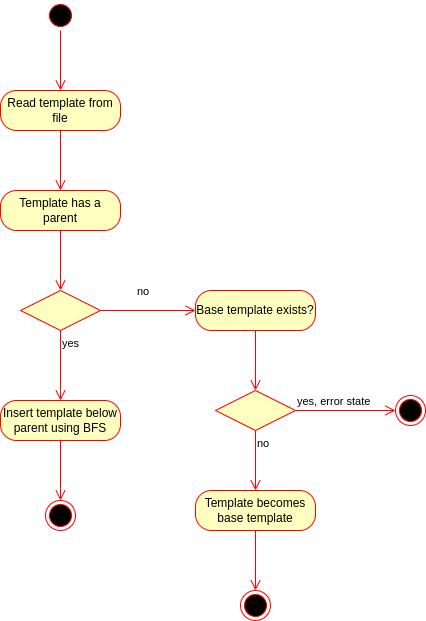
\includegraphics[scale=0.5]{insert_template_acty}
	\caption{Template insert operation}
	\label{fig:inserttemplate}
\end{figure}

\section{Keeping revision history}
In order to fulfill the ability to restore a template to a previous version a revision history is kept.


Design:
Each time a template is saved it is saved as a yaml file and committed in git.
A commit only modifies one file at a time.
A template can be reverted to an earlier commit.
Author information is entered at the login screen.
library available that implements porcelain functions:
https://github.com/go-git/go-git

Decision that still needs to be made:
Keep all templates in the same directory or keep them in separate ones.
Separate directories may be slightly more efficient due to the way git stores these but this may not matter at this scale nor make sense as there is only a single file for a template now.
It could be stored in the same directory.

\section{Camera interface}
The camera interface is a system component that sits between the template component and the cameras themselves. The purpose of this component
is to translate the settings from a template into an API call understood by the camera. Each camera can have a different API with potentially different interpretation of parameters.
While two camera's of the same brand may use the same API.
There still might be some slight differences between two models that are not completely compatible.
Instead of adding a new API that is tailored specifically to that model a provision is made to store information about the camera model inside the Camera struct.
This information could be used by the API to modify it's behavior for that particular model that still allows the use of the other functions of the API that are common to all models of the particular camera vendor.
This component maps the parameter from the template to an appropriate value for that camera.
In order for a camera to accept new parameters they require a form of authentication. All cameras being used to implement the prototype support both HTTP Basic and HTTP Digest authentication.
To successfully interface with the cameras one or both of these authentication methods must be supported by the camera interface component.

TODO Add activity diagram from notes here

\section{Translating generic parameters to camera specific values}
As an example of translating a generic parameter to a camera specific value the detection sensitivity parameter is used.
For the Hikvision camera this is a value that can be configured between 0 and 100 in increments of 20.
For the VCA camera this works by setting a number between 1 and 128.

Because these parameters may behave differently between camera manufacturers and individual models the template parameter is divided into a couple of presets. The presets are labeled as low, medium, high and ultra. These predefined levels are used by the Camera API to map a parameter to a specific value for that camera. These values are implemented in such a way that extra levels can be introduced and their values adjusted to fine tune a cameras behavior.

\section{Detecting differences between a template and actual configuration}
As stated in requirement B5 a capability must exit to detect if a camera still is still configured according to the parameters in the configuration.
To achieve this the CameraAPI has been split into three operations that split a configuration action into multiple steps.
The first operation is called Prepare, it pulls the current configuration from the camera and stores it for use by the other steps.
The Prepare operation must be executed each time an operation is to be done to a camera to ensure the systems has the latest configuration from the camera.
The other two operations are Configure and Compare.
The Compare operation uses the parameters from the template and compares these with the parameters from the camera.
If a mismatch exists the parameter being compared is added to a list which is displayed to the user to inform them of the actual and expected values of a parameter.
The Configure operation enumerates all parameters in the template associated with the camera and writes this configuration to the camera.
This way the CameraAPI can be run up to the point that it is ready to write the new parameters to the camera.
At that point it can be checked if any changes would be made and if so what parameters are affected.
The user can then be presented with both the parameter value in the template as the one that is read from the camera.

\section{User interface}
The components of the system can be managed through a web interface.
They will allow the user to create a new template and add parameters to it as seen in figure \ref{fig:templatewireframe}.
The user should also be able to manage the relations between templates as well as registering new cameras to be managed by the system (TBD still).
\begin{figure}[h!]
	\centering
	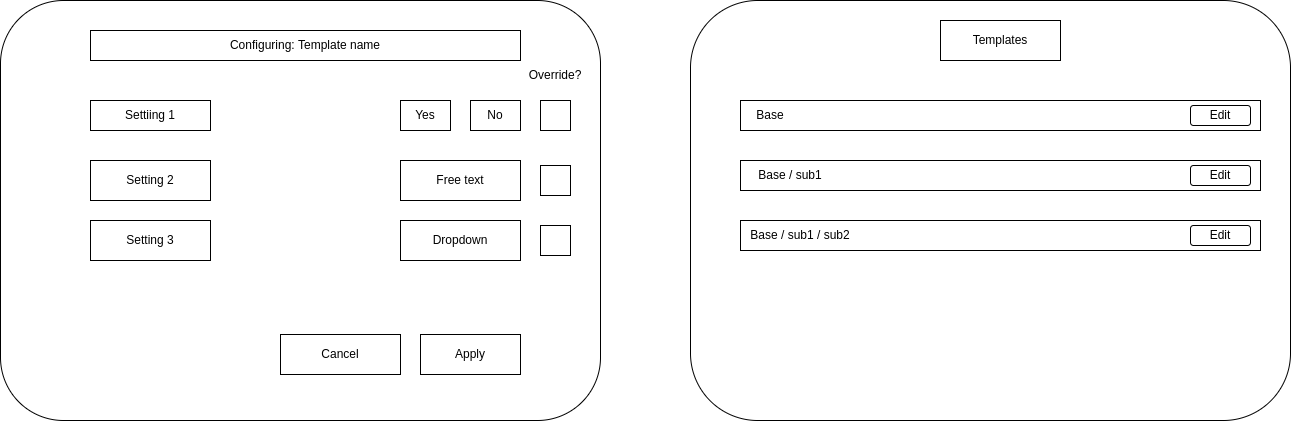
\includegraphics[scale=0.2]{wireframes}
	\caption{Template overview  wireframe}
	\label{fig:templatewireframe}
\end{figure}

\section{Design patterns}
TBD Integrate these where applicable instead of separately.

Design patterns are reusable solutions to commonly occurring software design problems. Design patterns are not ready made solutions that directly translate to machine readable code. Rather they are concepts that can be applied to solve a common problem in different situations. They may be seen as an intermediate between a programming paradigm (e.g. functional- or object-oriented programming) and
concrete algorithms. Design patterns can be divided in three categories, namely creational, behavioral and structural.

\subsection{Composite}
The composite pattern is a structural design pattern. With this design pattern objects can be grouped such that they are treated as a
single instance.

\subsection{Factory}
The factory method is a creational design pattern used for creating objects in a generic superclass that allows subclasses to change the
specific type of object that is created.
